%--------------------------------------------------------------------------
%	PACKAGES AND OTHER DOCUMENT CONFIGURATIONS
%--------------------------------------------------------------------------
\documentclass[11pt,a4paper]{article}
\usepackage[utf8]{inputenc}
\usepackage[francais]{babel}
\usepackage[T1]{fontenc}
\usepackage{amsmath}
\usepackage{amsfonts}
\usepackage{amssymb}
\usepackage{graphicx}
\usepackage{lmodern}
\usepackage[left=2cm,right=2cm,top=2.2cm,bottom=2.2cm]{geometry}

\usepackage{fancyhdr} % Required for custom headers
\usepackage{lastpage} % Required to determine the last page for the footer
\usepackage{extramarks} % Required for headers and footers
\usepackage[usenames,dvipsnames]{color} % Required for custom colors
\usepackage{graphicx} % Required to insert images
\usepackage{caption}
\usepackage{subcaption}
\usepackage{listings} % Required for insertion of code
\usepackage{courier} % Required for the courier font
\usepackage{verbatim}
\usepackage{multirow}
\usepackage{eurosym}
\usepackage[squaren,Gray]{SIunits}
\usepackage{url}
\usepackage{hyperref}

% Margins
%\topmargin=-0.45in
%\textwidth=6.5in
%\textheight=9.8in
\headsep=0.25in

% Set up the header and footer
%\pagestyle{fancy}
%\rhead{\firstxmark} % Top right header
%\lfoot{\lastxmark} % Bottom left footer
%\cfoot{} % Bottom center footer
%\rfoot{Page\ \thepage\ /\ \protect\pageref{LastPage}} % Bottom right footer
%\renewcommand\headrulewidth{0.3pt} % Size of the header rule
%\renewcommand\footrulewidth{0.3pt} % Size of the footer rule

\setlength\parindent{0pt} % Removes all indentation from paragraphs

%--------------------------------------------------------------------------
%	CODE INCLUSION CONFIGURATION
%--------------------------------------------------------------------------

\definecolor{MyDarkGreen}{rgb}{0.0,0.4,0.0} % This is the color used for comments
\lstloadlanguages{C} % Load C syntax for listings, for a list of other languages supported see: ftp://ftp.tex.ac.uk/tex-archive/macros/latex/contrib/listings/listings.pdf

\begin{document}
	
%--------------------------------------------------------------------------
%	TITLE PAGE
%--------------------------------------------------------------------------
\begin{titlepage}
\newcommand{\HRule}{\rule{\linewidth}{0.5mm}} % Defines a new command for the horizontal lines, change thickness here
\centering % Center everything on the page
 
%	HEADING SECTIONS
\null
\vspace{1cm}
\textsc{\Large Université Catholique de Louvain}\\[1cm] % Name of your university/college
\textsc{\large LINGI2141 \\[0.3cm] Computer Networks : Information transfert}\\[0.5cm] % Major heading such as course name
%\textsc{\large Minor Heading}\\[0.5cm] % Minor heading such as course title

%	TITLE SECTION

\HRule \\[0.4cm]
{ \LARGE \bfseries Project 1~: Reliable Transfer Protocol\\[0.4cm] % Title of your document
\large \bfseries Report} \\[0.4cm]

\HRule \\[0.5cm]
 
\begin{figure}[!h]
	\begin{center}
	%2048 × 1364
		\includegraphics[width=10cm]{images/cover.jpeg}
	\end{center}
\end{figure}

%	AUTHOR SECTION

\large
\begin{centering}
\end{centering}
{\begin{tabular}{lll}
\textsc{Legat} & Benoît & 4896 11 00\\
\textsc{Sedda} & Mélanie & 2246 11 00\\
\end{tabular}}
\\[1cm]

\normalsize
{\begin{tabular}{ll}
\textit{Teacher} : & Olivier Bonaventure\\
\textit{Assistants} : & Juan Antonio Cordero Fuertes\\
& Matthieu Baerts\\
& Raphael Bauduin\\
& David Lebrun\\
& Olivier Tilmans
\end{tabular}}
\\[1cm]

%	DATE SECTION

{\normalsize \today} % Date, change the \today to a set date if you want to be precise

\newpage

\end{titlepage}

%--------------------------------------------------------------------------
%	TABLE OF CONTENTS
%--------------------------------------------------------------------------
%
%\pagenumbering{gobble}
%\clearpage
%\thispagestyle{empty}
%\tableofcontents
%\clearpage
%\pagenumbering{arabic}

%--------------------------------------------------------------------------
%	CONTENT
%--------------------------------------------------------------------------

%--------------------------------------------------------------------------
%	IMPLEMENTATION CHOICES
%--------------------------------------------------------------------------
\section{Implementation choices}

\subsection{Sender}

We choose to create several agents responsible for different aspects of the sender, each one running in a different thread so that these different aspects can run in parallel. Theses agents communicate with each other via a mailbox system we implemented (we associated with each agent a linked list of messages).
\begin{itemize}
\item \textbf{Timer} This agent is responsible for everything related to the time. When another agent wants to launch an alarm that will expire at a certain time $t$, it delegates the work to Timer : it sends a message to Timer and the Timer will take care to prevent it once the alarm expired. This agent is useful both to implement the retransmission timer and to simulate the delays to send data and receive acknowledgments. For each $id$ in the sending buffer, there could be three alarms : one to simulate the delay to send the corresponding packet, another to simulate the delay to receive an acknowledgement (ack) for this packet and another to know when to retransmit the packet if no acknowledgment is received. Therefore, Timer uses an array of alarms whose size is equal to 3 times the maximum size of the sending buffer. The entries of this buffer at the slots $\equiv 0$ (mod $3$) are used for the delays of transmission of packets, the ones $\equiv 1$ (mod $3$) for the delays of transmissions of the acks and the one $\equiv 2$ (mod $3$) for the retransmission timers.
\item \textbf{Acker} This agent is the one who reads the socket. 
\item \textbf{Network Simulator} This agent is the one who actually send the packets to the receiver via the function \texttt{sendto()}. It keeps a linked lists of everything he has to sent. As soon as he receives a timeout message from the Timer, he looks for the expired packets in this list and sends them.
\item \textbf{Selective Repeat}  This agent is responsible to read the file and create packets that the Network Simulator will send. Let's notice that if the content of the file is a multiple of $512$ bytes then it creates a packet with no data in it to allow the sender to detect the end of the transmission. The Selective Repeat manages everything related to the sending window. It is held aware of the received acknowledgments by the Acker, which transmits the information to Network Simulator (with an id which is just useful for the Timer), which sends it to the Selective Repeat.
\end{itemize}
The Figure~\ref{sender} summarizes the interactions between those agents. Network Simulator knows that a packet is the last one when the length entry is $< 512$. When the ack corresponding to the sequence number of this packet is received by the Network Simulator, he says to Acker that he can stop. Then Selective Repeat, Timer and Network simulator also stop.

\begin{figure}[!h]
	\begin{center}
		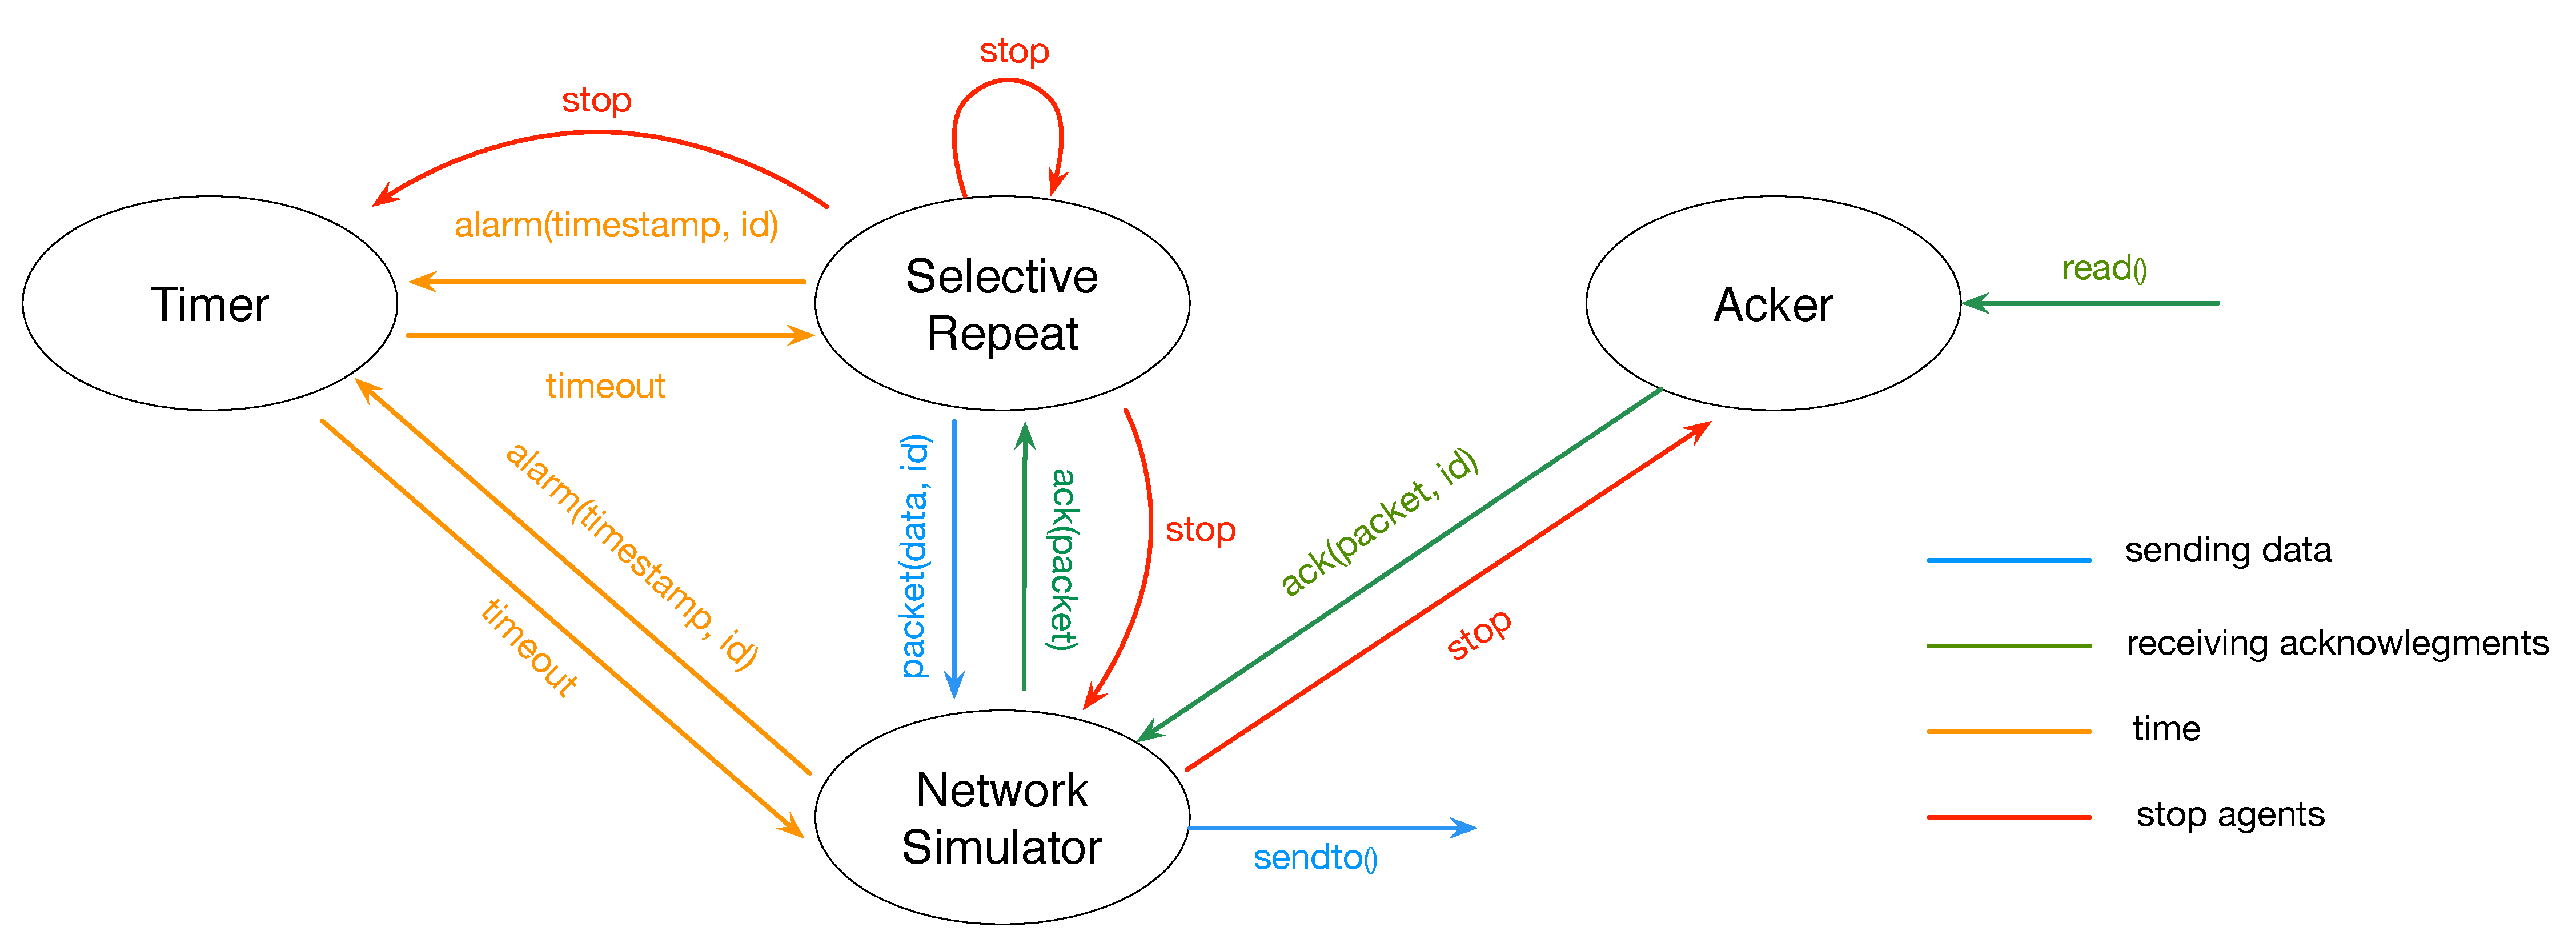
\includegraphics[width=18cm]{images/sender.eps}
		\caption{Agents modeling the sender}
		\label{sender}
	\end{center}
\end{figure}

\subsubsection{RTT}
We chose to take a RTT equal to 3 times the delay specified in the arguments of the sender. The RTT must be $> 2*$delay because it is the minimum delay between the transmission and reception of a packet and $3*$delay is the smaller value which is always an integer $>2*$delay.

\subsubsection{Clean exit in case of errors}
We took care to properly exit the sender in case of error. In \lstinline|error.c|, we defined that when an error occurs, we print a message according to \lstinline|errno|
and we set the flag \lstinline|panic| to \lstinline|true|. In \lstinline|agent.c|, before each message, if the \lstinline|panic| flag is set, the rest of the messages are ignored and the thread terminates. In \lstinline|sender.c|, we join each threads, close the file and exits with status \lstinline|EXIT_FAILURE|.

\subsubsection{Consideration of the variable size of the receiving window}

\subsection{Receiver}
The implementation of the receiver is more straightforward. We implemented a buffer to store out-of-sequence packets whose sequence numbers are in the receiving window. We thought of two ways to implement this buffer : create a linked list or create an array. The fist solution has the advantage to better manage the memory. Indeed, the size of the receiving window can change and with a linked list we can create a buffer whose size is really equal to the size of the receiving window. But this solution has a big drawback : the access of an element of a linked list is in $\mathcal{O}(n)$, where $n$ is the size of the list. Since we know the maximum size of the sending window and it is quite small ($31$ slots), it is better to simply create an array to have an access in $\mathcal{O}(1)$. Each slot of the buffer contains a boolean saying if it is empty or not and a corresponding packet. The receiver holds a variable \texttt{lastack} which corresponds to the sequence number of the last in-sequence packet that it has received (so $0 \leq lastack \leq 255$). The sequence number contained in an ack packet is then always equal to \texttt{lastack + 1 (mod 255)}. To avoid having to move some packets in the buffer when the window slides, we created a variable \texttt{lastack\_in\_window}, which goes from $0$ to $30$. The behavior of these two variables are similar. They are incremented in the same way but we work mod $256$ for \texttt{lastack} and mod $31$ for \texttt{lastack\_in\_window}. This variable allows us to ensure that a packet is mapped to the same slot of the buffer before and after the window slides by doing some appropriate modular computations.  We used the same trick for the sending window.

\begin{figure}[!h]
	\begin{center}
		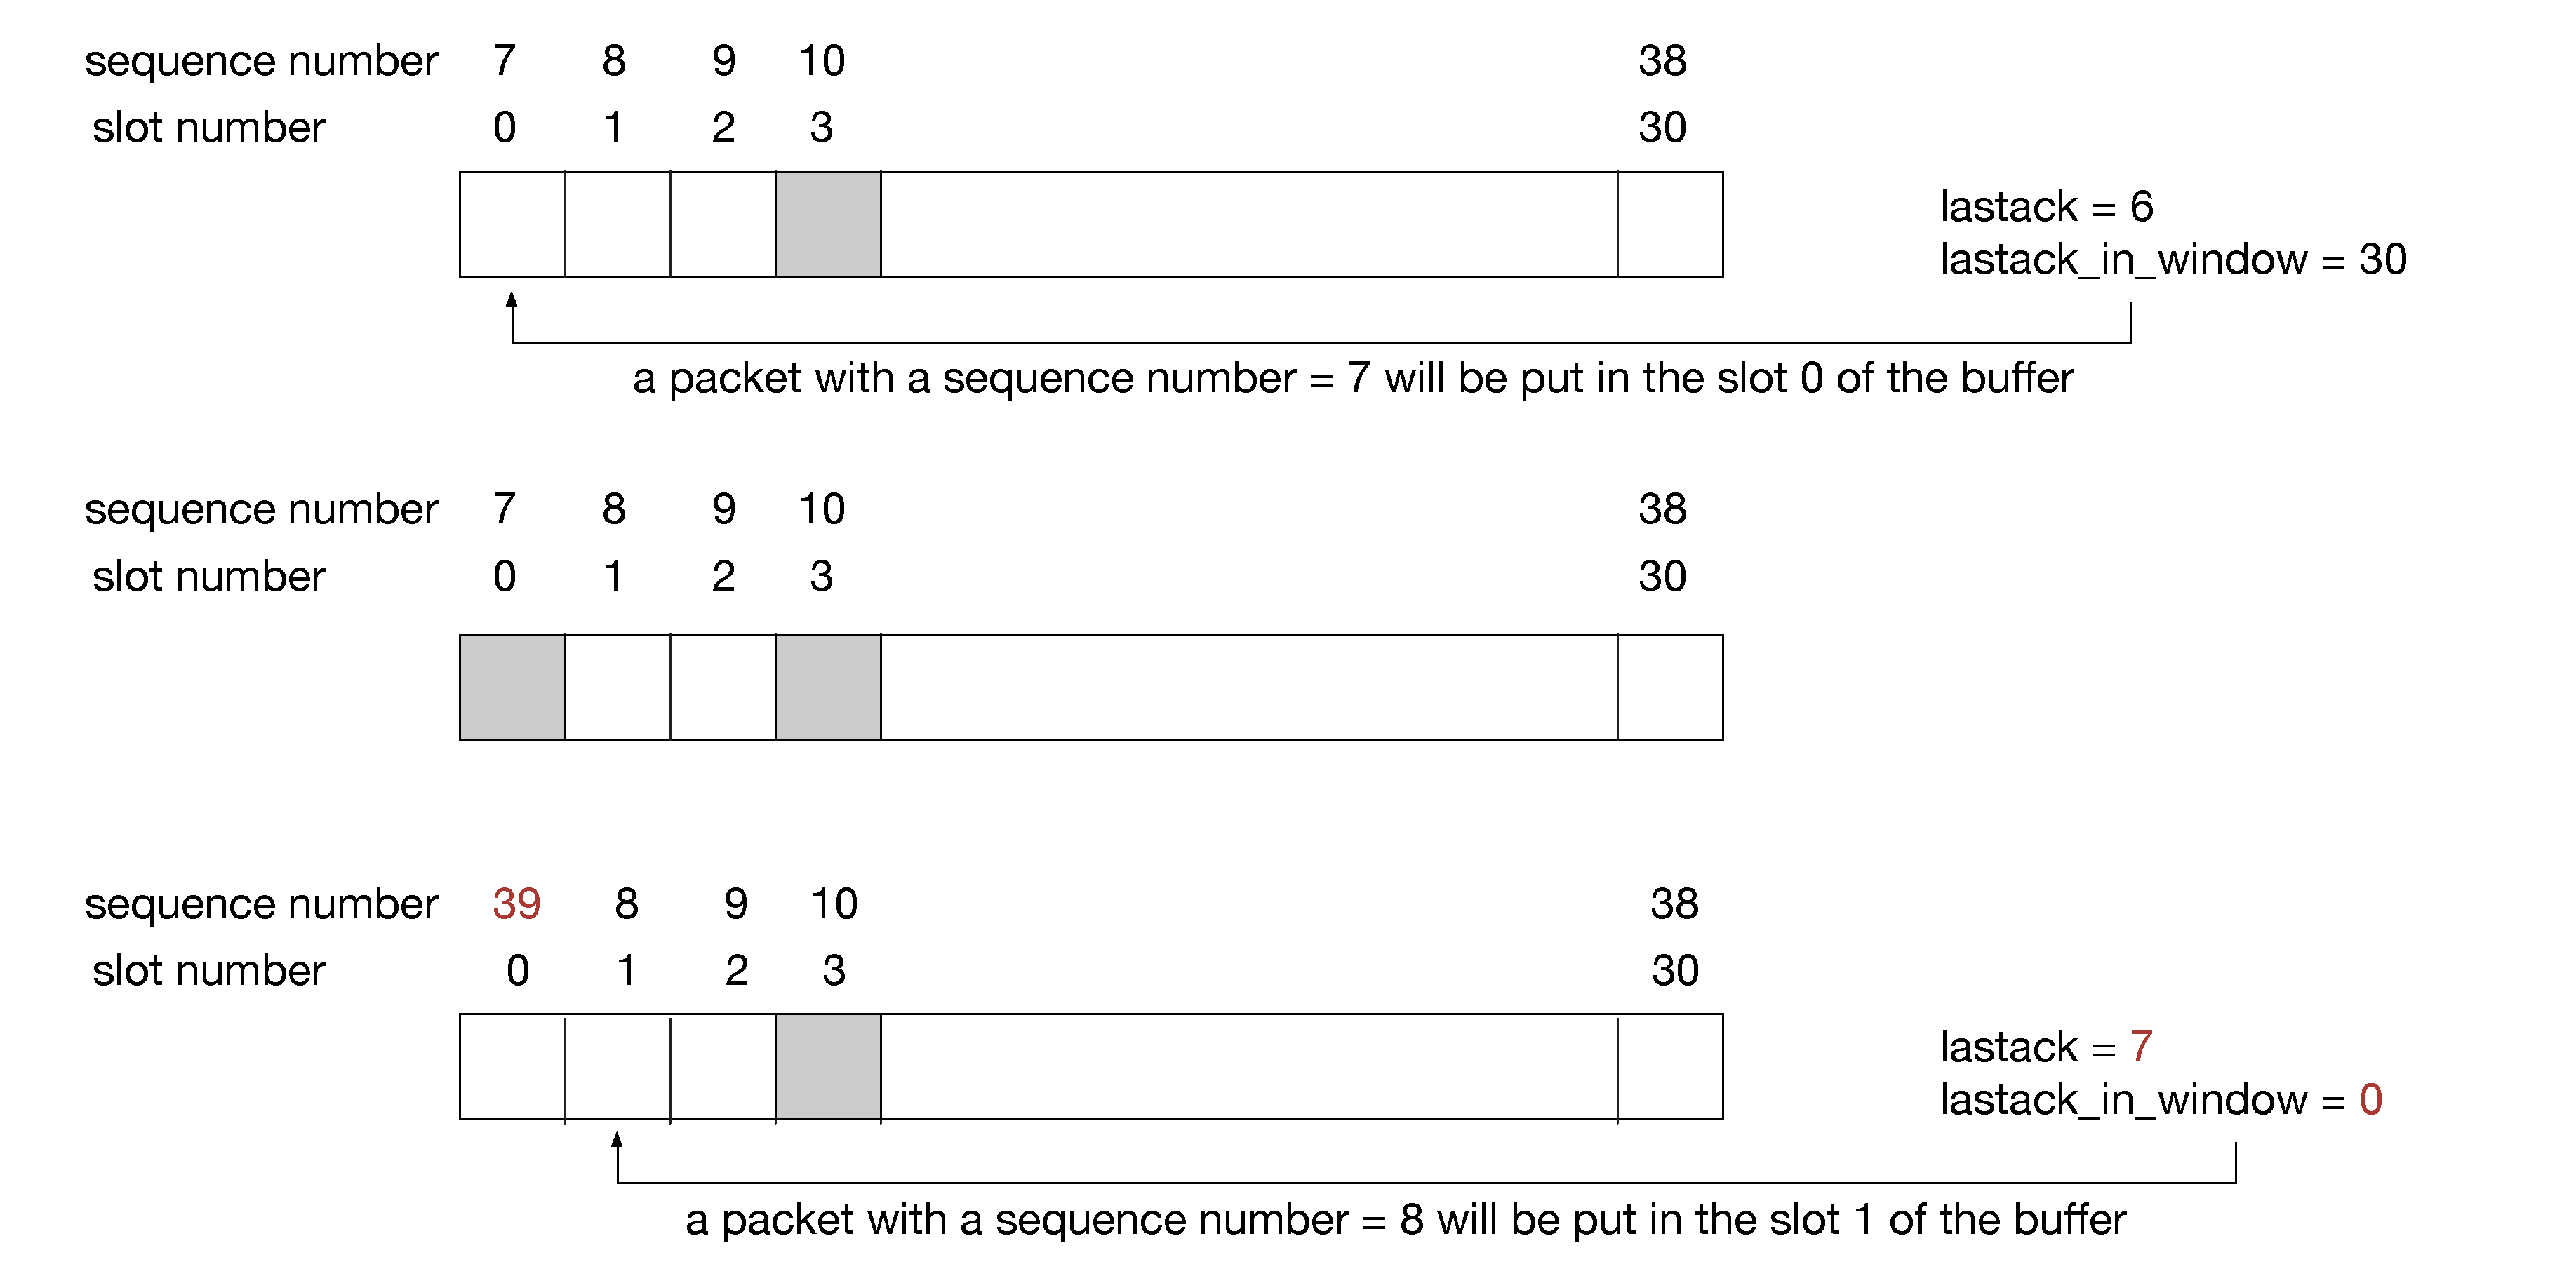
\includegraphics[width=15cm]{images/buffer.eps}
		\caption{Illustration of the behavior of the buffer when receiving a packet}
		\label{sender}
	\end{center}
\end{figure}
%--------------------------------------------------------------------------
%	LIMITATIONS
%--------------------------------------------------------------------------
\section{Limitations}

Our implementation suffers from some limitations.

\subsection{RTT optimization} The sender could update the RTT with respect to what it measures. If it sees that, on average, it receives an ack $x$ milliseconds after sending it, with $x << RTT$ (resp. $>>$), it could decrease (resp. increase) the value of the RTT. 

\subsection{Last packet}
When the receiver receives the last packet, it sends an ack back but it is possible that this acknowledgment gets lost. One idea is to force the receiver to wait a little bit. That way, the retransmission timer for this packet could expire, the packet could be retransmitted and the receiver would then retransmit one ack. But if the ack is not lost, then the receiver would block because of the \texttt{recvfrom()} operation. So, we just chose to close the receiver just after he sends the last ack. When the sender sees that the receiver is no longer listening, he also stops it's execution.

\subsection{Smart variation of the receiving window size}
One improvement of our implementation would be to really make the size of the receiving window vary. If the processor related to the receiver is slow, it would receive packets faster than it treats them. It would be better to ask the kernel how many packets the receiver still has the treat and if it sees that it can't follow, then it should then decrease to size of the window. That way, the sender would be informed that the receiver can't follow via the window size specified in the ack packets and it would decrease it's own window size to send less packet at once (without waiting for previous acks). 

%--------------------------------------------------------------------------
%	PERFORMANCE
%--------------------------------------------------------------------------
\section{Factors limiting the performance}

%--------------------------------------------------------------------------
%	INTEROPERABILITY TEST
%--------------------------------------------------------------------------
\section{Interoperability test }

\subsection{Derval-Gego}
\subsubsection{Our sender} grande nombre d'envoi du même packet

\subsection{Our receiver} Tout ok, bonne réception de fichier
    
\end{document}
